\documentclass{beamer}
\usetheme{Madrid}
\usepackage{pgfplots}
\pgfplotsset{compat=1.18}
\usetikzlibrary{arrows.meta}

% --- Colors -----------------------------------------------------------
\definecolor{slowc}{RGB}{40,110,220}   % slow wave
\definecolor{fastc}{RGB}{220,50,50}    % fast wave
\definecolor{tracec}{RGB}{255,210,40}  % oscilloscope trace
\definecolor{sqc}{RGB}{240,140,20}     % square wave

% --- Styles -----------------------------------------------------------
\pgfplotsset{
  % small plot without axes (for the "ingredients")
  mini/.style={
    width=3.2cm, height=2.0cm, axis lines=none,
    xmin=0, xmax=4*pi, ymin=-1.6, ymax=1.6,
    samples=200, domain=0:4*pi, scale only axis=false,
  },
  % instrument screen
  screen/.style={
    axis background/.style={fill=black!85},
    grid=major, grid style={green!35!black},
    xtick={0,1,...,10}, ytick={-2,-1,...,2},
    xticklabels={}, yticklabels={},
    major tick length=0pt,
    axis line style={black!60, line width=1.5pt},
    label style={font=\footnotesize},
    xlabel style={yshift=6pt}, ylabel style={yshift=-6pt},
  },
  timescreen/.style={
    screen, xmin=0, xmax=10, ymin=-2, ymax=2,
    xlabel={time $\rightarrow$}, ylabel={voltage},
    samples=300, domain=0:10,
  },
  freqscreen/.style={
    screen, xmin=0, xmax=10, ymin=-2, ymax=2,
    xlabel={frequency $\rightarrow$}, ylabel={level},
  },
  peak/.style={line width=3pt, mark=*, mark size=2.5pt, mark indices={2}},
}

\begin{document}

% ======================================================================
\begin{frame}{Same signal -- two ways to look at it}

\centering
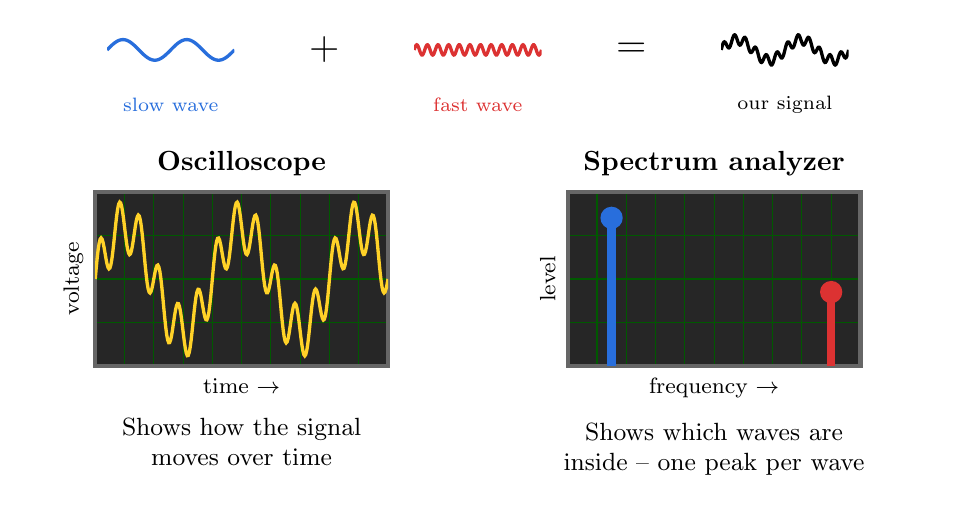
\begin{tikzpicture}

  % ---- Top: the signal is made of two "ingredients" ------------------
  \begin{axis}[mini, name=slow, at={(0cm,0cm)}, anchor=center]
    \addplot[slowc, very thick] {sin(deg(x))};
  \end{axis}
  \node[font=\Large\bfseries] at (1.95,0) {$+$};
  \begin{axis}[mini, name=fast, at={(3.9cm,0cm)}, anchor=center]
    \addplot[fastc, very thick] {0.5*sin(deg(6*x))};
  \end{axis}
  \node[font=\Large\bfseries] at (5.85,0) {$=$};
  \begin{axis}[mini, name=sum, at={(7.8cm,0cm)}, anchor=center]
    \addplot[black, very thick] {sin(deg(x)) + 0.5*sin(deg(6*x))};
  \end{axis}
  \node[font=\scriptsize, slowc] at (0,-0.7) {slow wave};
  \node[font=\scriptsize, fastc] at (3.9,-0.7) {fast wave};
  \node[font=\scriptsize]        at (7.8,-0.7) {our signal};

  % ---- Bottom: the two instruments -----------------------------------
  \begin{axis}[timescreen, name=scope, width=5.3cm, height=3.8cm,
               at={(0.9cm,-1.8cm)}, anchor=north,
               title={\textbf{Oscilloscope}}, title style={yshift=-4pt}]
    \addplot[tracec, very thick]
      {1.2*sin(deg(0.5*pi*x)) + 0.6*sin(deg(3*pi*x))};
  \end{axis}

  \begin{axis}[freqscreen, name=sa, width=5.3cm, height=3.8cm,
               at={(6.9cm,-1.8cm)}, anchor=north,
               title={\textbf{Spectrum analyzer}}, title style={yshift=-4pt}]
    \addplot[peak, slowc] coordinates {(1.5,-2) (1.5,1.4)};
    \addplot[peak, fastc] coordinates {(9,-2) (9,-0.3)};
  \end{axis}

  % ---- One-line captions ---------------------------------------------
  \node[font=\small, text width=5.2cm, align=center, below=2pt, execute at begin node={\hyphenpenalty=10000}]
    at (scope.below south) {Shows \alert{how the signal moves} over time};
  \node[font=\small, text width=5.2cm, align=center, below=2pt, execute at begin node={\hyphenpenalty=10000}]
    at (sa.below south) {Shows \alert{which waves} are inside -- one peak per wave};

\end{tikzpicture}

\end{frame}

% ======================================================================
\begin{frame}{Examples}

\centering
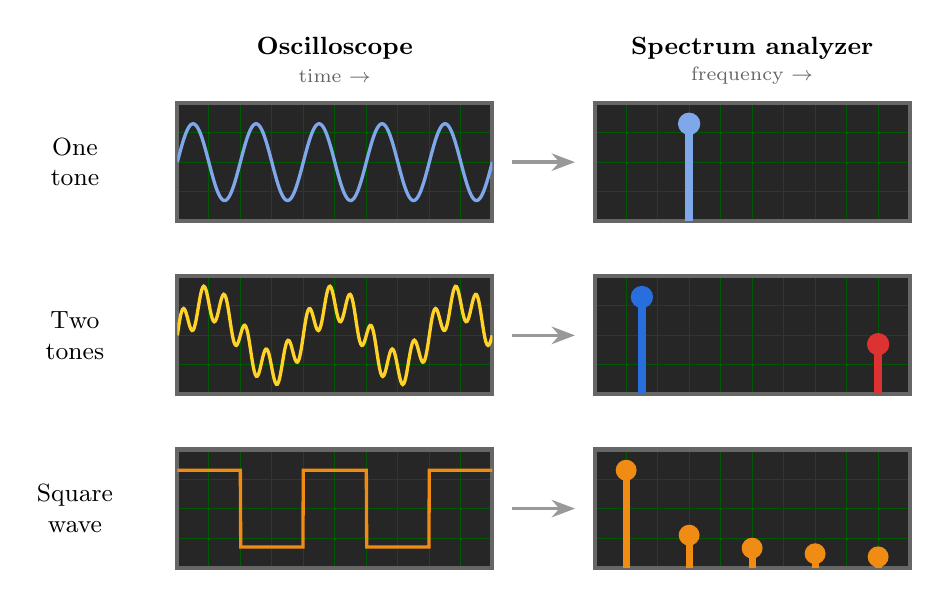
\begin{tikzpicture}
  \pgfplotsset{
    ex/.style={scale only axis, width=4.0cm, height=1.5cm, xlabel={}, ylabel={}},
  }

  % column headers
  \node[font=\bfseries\small] at (3.3,0.35) {Oscilloscope};
  \node[font=\bfseries\small] at (8.6,0.35) {Spectrum analyzer};
  \node[font=\scriptsize, black!60] at (3.3,0.0)  {time $\rightarrow$};
  \node[font=\scriptsize, black!60] at (8.6,0.0)  {frequency $\rightarrow$};

  % ---- Row 1: one tone -------------------------------------------------
  \node[font=\small, align=center] at (0,-1.1) {One\\tone};
  \begin{axis}[timescreen, ex, at={(3.3cm,-1.1cm)}, anchor=center]
    \addplot[slowc!60!white, very thick] {1.3*sin(deg(pi*x))};
  \end{axis}
  \draw[-{Stealth}, very thick, black!40] (5.55,-1.1) -- (6.35,-1.1);
  \begin{axis}[freqscreen, ex, at={(8.6cm,-1.1cm)}, anchor=center]
    \addplot[peak, slowc!60!white] coordinates {(3,-2) (3,1.3)};
  \end{axis}

  % ---- Row 2: two tones ------------------------------------------------
  \node[font=\small, align=center] at (0,-3.3) {Two\\tones};
  \begin{axis}[timescreen, ex, at={(3.3cm,-3.3cm)}, anchor=center]
    \addplot[tracec, very thick]
      {1.1*sin(deg(0.5*pi*x)) + 0.6*sin(deg(3*pi*x))};
  \end{axis}
  \draw[-{Stealth}, very thick, black!40] (5.55,-3.3) -- (6.35,-3.3);
  \begin{axis}[freqscreen, ex, at={(8.6cm,-3.3cm)}, anchor=center]
    \addplot[peak, slowc] coordinates {(1.5,-2) (1.5,1.3)};
    \addplot[peak, fastc] coordinates {(9,-2) (9,-0.3)};
  \end{axis}

  % ---- Row 3: square wave ---------------------------------------------
  \node[font=\small, align=center] at (0,-5.5) {Square\\wave};
  \begin{axis}[timescreen, ex, at={(3.3cm,-5.5cm)}, anchor=center, samples=801]
    \addplot[sqc, very thick] {sin(deg(0.5*pi*x)) >= 0 ? 1.3 : -1.3};
  \end{axis}
  \draw[-{Stealth}, very thick, black!40] (5.55,-5.5) -- (6.35,-5.5);
  \begin{axis}[freqscreen, ex, at={(8.6cm,-5.5cm)}, anchor=center]
    \foreach \n in {1,3,5,7,9} {
      \pgfmathsetmacro\h{-2+3.3/\n}
      \edef\temp{\noexpand\addplot[peak, sqc, line width=2.5pt]
        coordinates {(\n,-2) (\n,\h)};}
      \temp
    }
  \end{axis}

\end{tikzpicture}

\end{frame}

\end{document}
